\chapter{Metodologia de Desenvolvimento}
\label{chap:metodologia}

Neste capítulo será detalhado o trabalho proposto por essa monografia, um estudo sobre a utilização das instâncias EC2 F1 como recurso didático para a disciplina de Sistemas Eletrônicos Digitais Reconfiguráveis (SEDR). Serão apresentadas a metodologia utilizada, todas as práticas realizadas e as ferramentas utilizadas.

\section{Metodologia Utilizada}\label{sec: metodologia-utilizada}

As metodologia adotada para a execução deste trabalho pode ser descrita pelas etapas mostradas na Figura \ref{fig:metodologia}:



\begin{figure}[htb!] 
   	    \captionsetup{width=15cm}%Da mesma largura que a figura
		\Caption{\label{fig:metodologia} Metodologia}
		\UFCfig{}{
			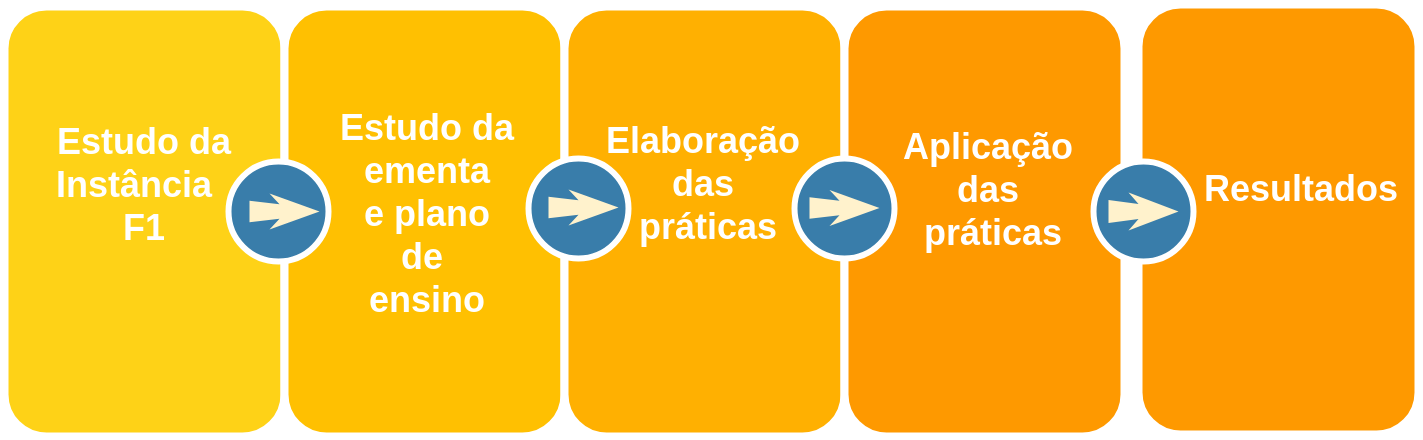
\includegraphics[width=16cm]{figuras/metodologia.png}
		}{
			\Fonte{Próprio Autor.}
	}		
\end{figure}
    
\begin{enumerate}
    \item \textbf{Estudo da Instância F1:} Primeiramente, foi realizado um estudo das instâncias EC2 F1 com o intuito de identificar as possibilidades que esse recurso poderia oferecer para o seu uso no ensino de FPGA.
    
    \item \textbf{Estudo da ementa e plano de ensino da Disciplina de SEDR:} Em seguida, deu-se início ao estudo da ementa e do plano de ensino da disciplina de SEDR para que a utilização das instâncias EC2 F1 fosse adequada da melhor forma possível ao plano de ensino.
    
    \item \textbf{Elaboração das práticas:} Baseando-se nos estudos já realizados e na documentação da Amazon Web Services, as práticas de laboratório foram idealizadas de forma a oferecer um conhecimento geral do processo de desenvolvimento de aplicações para FPGA com o serviço EC2 F1.
    
    \item \textbf{Aplicação das práticas:} Após a elaboração e testes das práticas, iniciou-se a fase de aplicação em laboratório.
    
    \item \textbf{Resultados:} Finalmente, nesta última etapa da metodologia foi analisada a eficácia do uso das instâncias EC2 F1 como recurso didático para a disciplina de SEDR através da aplicação das práticas e de análise de questionários respondidos pelos alunos ao final de cada prática.
	  
\end{enumerate}

  
\section{Contextualização}\label{sec: contextuaizacao}

O trabalho foi realizado no Departamento de Teleinformática da Universidade Federal do Ceará. As práticas foram aplicadas em dois laboratórios deste mesmo departamento para alunos de graduação.

As práticas foram aplicadas na disciplina de SEDR, que é um componente optativo da estrutura curricular do Curso de Graduação em Engenharia de Computação e é ofertada no sétimo semestre da graduação. A mesma possui  uma carga horária de 64 horas (vide ANEXO A - Ementa de SEDR) e tinha o total de 8 alunos matriculados. 

De acordo com a ementa, a carga horária total da disciplina é dividida igualmente entre teoria e prática, ou seja, são utilizadas 32 horas para a teoria e 32 horas para a pŕatica. A carga horária reservada para a  aplicação das práticas desenvolvidas neste trabalho foi de 10 horas, dessa quantidade, 2 horas foram utilizadas para uma aula teórica sobre a Amazon Web Services e o serviço EC2 F1 e as 8 horas restantes foram reservadas para a aplicação das práticas, levando em consideração apenas as atividades desenvolvidas no laboratório durante o horário da aula.

As práticas foram realizadas no Laboratório de Informática (LI) e no Laboratório de Hardware do Departamento de Teleinformática. No primeiro, foram realizadas as práticas 1 e 2 que usam o acesso remoto as instâncias F1. As práticas 3 e 4 foram realizadas no Laboratório de Hardware, pois se utilizou máquinas virtuais, disponíveis nesse laboratório, que continham o kit de desenvolvimento da AWS,o HDK e o SDK, e o ambiente de desenvolvimento da Xilinx SDSoC, que contém o Vivado com uma licença específica para a FPGA Virtex UltraScale+ VU9P, permitindo  o desenvolvimento local (on premises) das pŕaticas.

\section{Ferramentas Utilizadas}\label{sec: ferramentas}

Esta seção detalha as ferramentas que foram utilizadas para a realização das atividades de labotório.

\subsection{Software}\label{sec: software}

\subsubsection{AWS CLI}\label{sec: aws-cli}


\subsubsection{GitHub}\label{sec: github}


\subsubsection{Vivado}\label{sec: vivado}

\subsubsection{VMware}\label{sec: vmware}


\subsection{Hardware}\label{sec: Hardware}

O hardware utilizado foram os computadores dos próprios laboratórios.